\chapter{Project Structure}
\label{cha:project_structure}
This chapter shows the structure of an project which implements the previously discussed authentication mechanisms.
This chapter aims to clarify the interactions of the components which are needed to implement the service-to-service security.
The visualizations of this chapter are based on a microservice backend for a flea market app.
The backend is implemented in C\# using the ASP.NET framework.

\section{Components}
The components of the example deployment are shown in figure~\ref{fig:deployment_structure}. 
It consists of the following parts:
\begin{description}
	\item[Android App:] The Android App is the User Interface for the client to access the functionalities of the service.
		The requests sent by the Android App are sent in beyond of the user.
	\item[Firebase Authentication:] The Firebase Authentication service is responsible for validating the access tokens wich are transferred by the users.
	\item[API Gateway:] The API Gateway is the only entry point to the deployment.
		Therefore the API Gateway is the only component which directly communicates to the Android App.
	\item[AdService:] The AdService is one service of the deployment.
		It is responsible to manage all ads offered to the users of the app.
	\item[UserService:] The AdService is the service which is responsible for managing the data of the users.
\end{description}

\begin{figure}
	\centering
	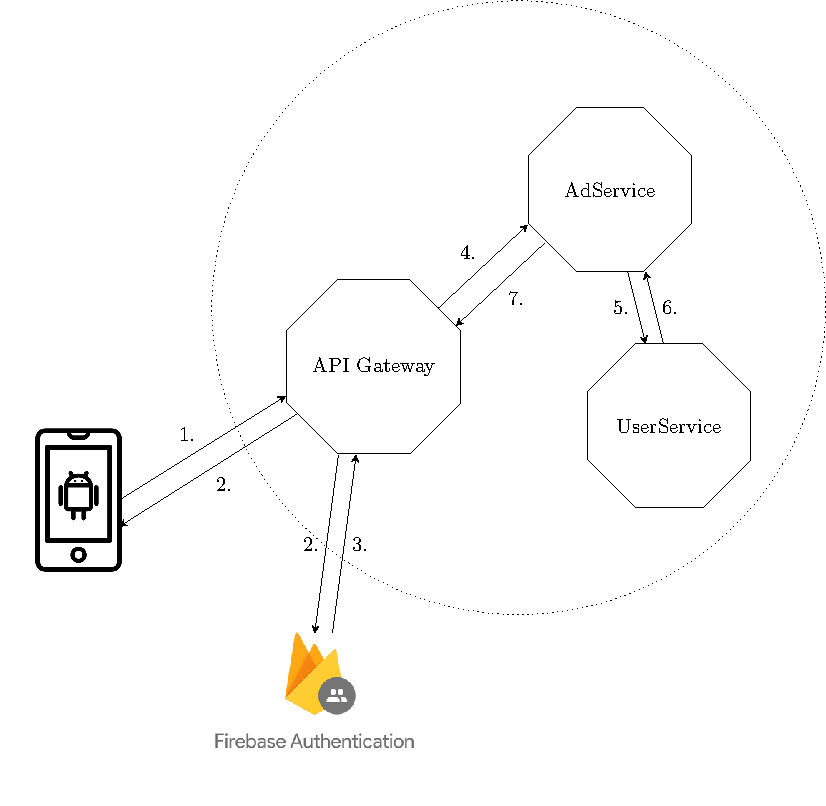
\includegraphics{images/project-structure/TikZ_structure.pdf}
	\caption{Structure of the deployment}
	\label{fig:deployment_structure}
\end{figure}

\section{Workflow using mTLS}

\begin{enumerate}
	\item The client sends an API request to the Microsoft API Gateway using an Android App.
		The client communicates with the API Gateway using HTTPS.
		Therefore the server is authenticated to the client using TLS.
		The client is authenticated to the server by embedding an firebase access token within the Authorization header.
	\item The API Gateway receives the request from the client and has to check the provided access token.
		The token is validated using an token validation service provided by firebase.
		If the token is invalid, the client has to retrieve a new token an start from the beginning.
		When the client provided an valid access token, the request of the client is forwarded to the "AdService".
		The communication between the API Gateway and the "AdService" is secured using mTLS.
		This means both the API Gateway and the AdService have to present a valid certificate signed by a trusted CA.
	\item The request from the client is then processed on the "AdService".
		Since the "AdService" needs information about the users which are the owners of the ads, it needs to communicate with the "UserService".
		The communication between the "UserService" and the "AdService" is also protected using mTLS.
	\item When the "UserService" processed the request from the "AdService", it responds with the expected result.
		The response does not require to present the certificates again, since TCP connection between the "AdService" and the "UserService" is still present.
	\item The "AdService" then processes the response from the "UserService" and sends its request to the API Gateway, again using the opened TCP connection.
	\item The API Gateway forwards the response from the "AdService" to the Android App.
		This connection is still secured using TLS and not mTLS.
		It would be possible to secure the communication between the API Gateway and the client using certificate.
		This mechanism is called Client Certificate Authentication.
	\item The App can now process the response and present the requested information to the user.
\end{enumerate}

\section{Workflow using self signed JWT}
